\section{Results}
\label{sec:results}

The optimization run reduced the cost of the objective function from the initialized value of of \$\num{2655.7} to an optimized value of \$\num{1526.5}. The components of the initialized and optimized objective function costs are shown in \cref{table:optimal-costs}.
The proposed model improves upon a simple priority-based heuristic by allowing the optimizer to minimize the operating cost by pumping water or BSS charging or some of both.


\begin{table}[t]
	\caption{Objective Function Components}
	\label{table:optimal-costs}
	\centering
	\begin{tabular}{lS[table-format=5.1]S[table-format=5.1]}
		\toprule
		   & {Initialized}  & {Optimized} \\
		   &  {(\$, 2020)}     & {(\$, 2020)} \\
		\midrule
		Grid energy cost  &  2448.1  &  1192.4 \\
		Battery use cost  &  198.6  &  326.1 \\
		Inadequate water cost  & 0.0  &  0.0 \\
		Battery mode switching cost  &  8.0  &  7.0 \\
		Pump switching cost  &  1.0  &  2.0 \\
		\midrule
		TOTAL  &  2655.7  &  1526.5 \\
		\bottomrule		
	\end{tabular}
\end{table}

%Figures \ref{fig:pv-side-power} - \ref{fig:water-used} show the results of the optimization run.


\begin{figure}[t]
	\centering
	\includegraphics[page=2, clip, trim=0.05in 2.2in 7.2in 0.15in, width=1.0\columnwidth]{optimization_plots}
	\caption{PV-Side Power}
	\label{fig:pv-side-power}
\end{figure}

\Cref{fig:pv-side-power} shows the power on the PV and BSS side of the microgrid.
Due to the relative ratings of the PV array, Pump 2, and the BSS, on the sunny days (24 and 26 February), the full available PV power is not able to be used.
The optimal operation does not strictly prefer pumping water or charging the BSS.
Instead, the BSS is charged enough to prevent the hybrid inverter from switching back to the grid.


\begin{figure}[t]
	\centering
	\includegraphics[page=2, clip, trim=0.03in 0.55in 7.2in 2.3in, width=1.0\columnwidth]{optimization_plots}
	\caption{Grid-Side Power}
	\label{fig:grid-side-power}
\end{figure}

\begin{figure}[t]
	\centering
	% trim=left botm right top
	\includegraphics[page=2, clip, trim=3.7in 2.7in 3.55in 0.15in, width=1.0\columnwidth]{optimization_plots}
	\caption{BSS Energy Stored}
	\label{fig:bss-energy}
\end{figure}

\Cref{fig:grid-side-power} shows the power on the grid side of the microgrid.
On the first day (24 February), the hybrid inverter starts initially connected to the grid.
As shown in \cref{fig:bss-energy}, once the BSS is recharged by PV during the day, the hybrid inverter switches to the PV/BSS source and is able to supply the load for the rest of the modeled period.
The largest load on the grid is Pump 1, which optimally runs during the nighttime hours where time-of-day electrical rates are cheapest.


%\begin{figure}[t]
%	\centering
%	% trim=left botm right top
%	\includegraphics[page=4, clip, trim=3.3in 0.15in 3.9in 2.35in, width=1.0\columnwidth]{optimization_demo}
%	\caption{BSS Power (Charging \& Discharging)}
%	\label{fig:bss-power}
%\end{figure}
%
%\Cref{fig:bss-power} shows the charging and discharging power to the BSS.
%As one would expect, it follows a pattern of charging during the part of the day in which PV energy is available and discharging to meet load during the dark period.


\begin{figure}[t]
	\centering
	% trim=left botm right top
	\includegraphics[page=2, clip, trim=7.2in 2.9in 0.05in 0.15in, width=1.0\columnwidth]{optimization_plots}
	\caption{Water Stored}
	\label{fig:water-level}
\end{figure}

%\begin{figure}[t]
%	\centering
%	% trim=left botm right top
%	\includegraphics[page=4, clip, trim=7.2in 1.3in 0.1in 1.7in, width=1.0\columnwidth]{optimization_demo}
%	\caption{Water Used}
%	\label{fig:water-used}
%\end{figure}

\Cref{fig:water-level} shows the water level in the two reservoirs.
% while \cref{fig:water-used} shows the water usage from each reservoir throughout the day.
Since the efficiency of water usage is highest at night, the optimal operation releases water during the nighttime hours.


